\documentclass[dvipdfmx]{jsarticle}

\title{個人レベルでGithubを使う}
\author{Seiichi Nukayama}
\date{2021-07-09}
\usepackage{tcolorbox}
\usepackage{color}
\usepackage{listings, plistings}

% Java
\lstset{% 
  frame=single,
  backgroundcolor={\color[gray]{.9}},
  stringstyle={\ttfamily \color[rgb]{0,0,1}},
  commentstyle={\itshape \color[cmyk]{1,0,1,0}},
  identifierstyle={\ttfamily}, 
  keywordstyle={\ttfamily \color[cmyk]{0,1,0,0}},
  basicstyle={\ttfamily},
  breaklines=true,
  xleftmargin=0zw,
  xrightmargin=0zw,
  framerule=.2pt,
  columns=[l]{fullflexible},
  numbers=left,
  stepnumber=1,
  numberstyle={\scriptsize},
  numbersep=1em,
  language={Java},
  lineskip=-0.5zw,
  morecomment={[s][{\color[cmyk]{1,0,0,0}}]{/**}{*/}},
}
\usepackage{url}
% \usepackage[dvipdfmx]{graphicx}
\usepackage[dvipdfmx]{hyperref}
\usepackage{amsmath, amssymb}
\usepackage{itembkbx}
\usepackage{eclbkbox}	% required for `\breakbox' (yatex added)
\usepackage{enumerate}
\usepackage{setspace}
\fboxrule=0.5pt
\parindent=1em
\begin{document}

%\anaumeと入力すると穴埋め解答欄が作れるようにしてる。\anaumesmallで小さめの穴埋めになる。
\newcounter{mycounter} % カウンターを作る
\setcounter{mycounter}{0} % カウンターを初期化
\newcommand{\anaume}[1][]{\refstepcounter{mycounter}{#1}{\boxed{\phantom{aa}\themycounter \phantom{aa}}}} %穴埋め問題の空欄作ってる。
\newcommand{\anaumesmall}[1][]{\refstepcounter{mycounter}{#1}{\boxed{\tiny{\phantom{a}\themycounter \phantom{a}}}}}%小さい版作ってる。色々改造できる。

%% 修正時刻: Fri Jul  9 12:01:07 2021


\section{Eclipseで Github を使う(プロジェクト編)}


\subsection{EclipseのプロジェクトをGitで管理する}

\subsubsection{新しいGitリポジトリをつくる}

自分のGitHubにアクセスし、新しくリポジトリを作成する。

\begin{enumerate}
 \item リポジトリ名 --- indean-poker
 \item Description --- Indean Poker Game of Servlet\_JSP
 \item mode --- Private
 \item Add a README file --- Check!
 \item Add .gitignore --- Check! --- Javaを選択
 \item Choose a lisence --- Check! --- MIT Lisence
\end{enumerate}

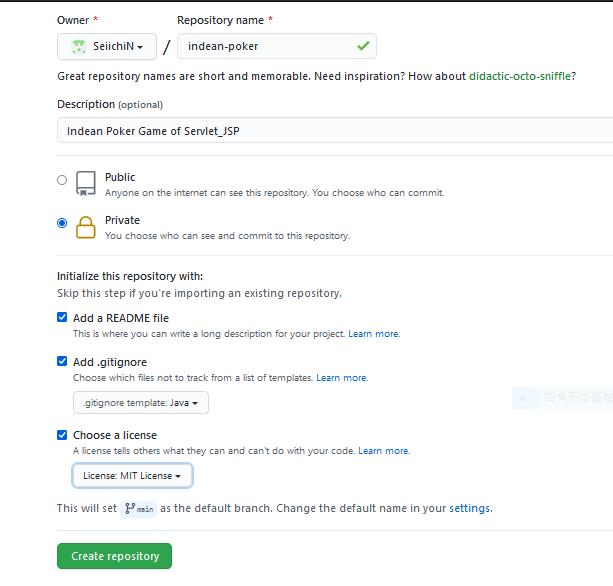
\includegraphics[width=12cm]{img/21-git-new.png}

リポジトリができたら、そのURLをコピーする。

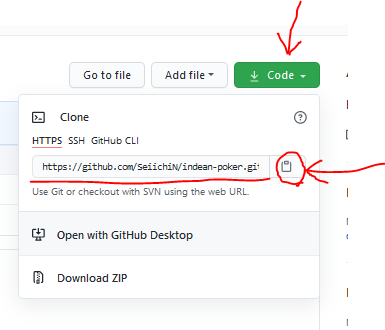
\includegraphics[width=12cm]{img/22-git-url.png}


\subsubsection{Eclipseのワークスペースで git clone}

現在使っているワークスペースにクローンすることにする。

sourcetree を起動し、ファイルメニューから「新規/クローンを作成する」
を選択する。

クローンを作成するウィンドウが開くので、上から順に以下のように指定する。

\begin{enumerate}
 \item GitHubでコピーしたURLを貼り付ける。
 \item Eclipseのワークスペース$+$indean-poker \\
       たとえば C:\yen pleiades\yen workspace \yen indean-poker となる。
 \item 名前 --- indean-poker
 \item Local Folder --- ルート
\end{enumerate}

\textgt{クローン} をクリックして実行。

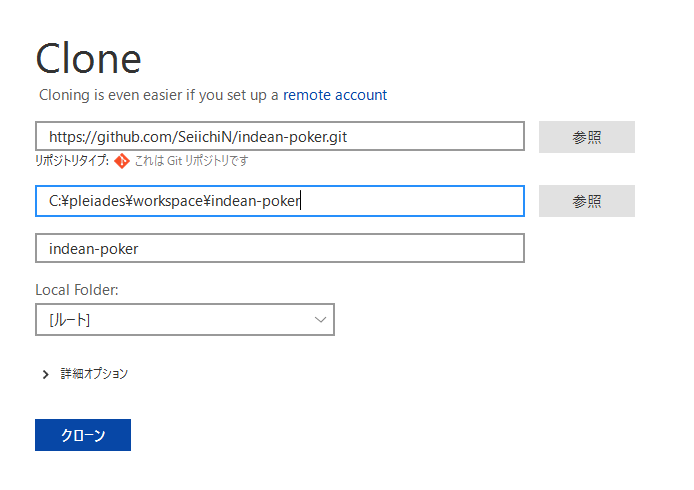
\includegraphics[width=12cm]{img/23-clone.png}

これで、\textsf{C:\yen pleiades\yen workspace} に \textsf{indean-poker}の
フォルダができているはず。

\subsubsection{Eclipseで新規動的Webプロジェクトを作成}

Eclipse でワークスペースを開き、以下のように動的Webプロジェクトを作成する。

\begin{tabular}{|l|l|}
 \hline
 プロジェクト名 & indean-poker \\ \hline
 ターゲットランタイム & Tomcat9 あるいは Tomcat8 \\ \hline
 動的Webモジュール & 4.0 あるいは 3.1 \\ \hline
 ソースフォルダー & src \\ \hline
 Webコンテンツディレクトリ & WebContent \\ \hline
\end{tabular}

とりあえず、以下のコードを入力する。

\begin{lstlisting}[caption=/WebContent/index.jsp]
 <%@ page language="java" contentType="text/html; charset=UTF-8"
    pageEncoding="UTF-8"%>
<!DOCTYPE html>
<html>
<head>
<meta charset="UTF-8">
<title>インディアン・ポーカー</title>
</head>
<body>
	<h1>インディアン・ポーカー</h1>
	<form action="<%=request.getContextPath() %>/play" method="post">
		<input type="hidden" name="mode" value="start">
		<input type="submit" value="札をひく">
	</form>
</body>
</html>
\end{lstlisting}

\begin{lstlisting}[caption=src/model/Card.java]
package model;

import java.io.Serializable;

public class Card implements Serializable {
	private static final long serialVersionUID = 1L;
	private String suit;
	private int number;

	public Card () {}
	public Card (String suit, int number) {
		this.suit = suit;
		this.number = number;
	}

	public String toString() {
		return suit + ":" + number;
	}

	public String getSuit() {
		return suit;
	}

	public void setSuit(String suit) {
		this.suit = suit;
	}

	public int getNumber() {
		return number;
	}

	public void setNumber(int number) {
		this.number = number;
	}
}
\end{lstlisting}


\begin{lstlisting}[caption=src/servlet/Play.java]
package servlet;

import java.io.IOException;
import java.util.HashSet;
import java.util.Set;

import javax.servlet.Servlet;
import javax.servlet.ServletConfig;
import javax.servlet.ServletContext;
import javax.servlet.ServletException;
import javax.servlet.annotation.WebServlet;
import javax.servlet.http.HttpServlet;
import javax.servlet.http.HttpServletRequest;
import javax.servlet.http.HttpServletResponse;

import model.Card;
import util.Const;

@WebServlet("/play")
public class Play extends HttpServlet {
	private static final long serialVersionUID = 1L;

	protected void doPost(HttpServletRequest request, HttpServletResponse response) throws ServletException, IOException {
		request.setCharacterEncoding("UTF-8");
		String mode = request.getParameter("mode");
		if (! mode.equals("start")) {
			response.sendRedirect("/index.jsp");
			return;
		}

		Card card = new Card("club", 12);
		request.setAttribute("card", card);
		request.getRequestDispatcher("/WEB-INF/jsp/play.jsp").forward(request, response);

	}

}
\end{lstlisting}

\begin{lstlisting}
<%@ page language="java" contentType="text/html; charset=UTF-8"
    pageEncoding="UTF-8"%>
<!DOCTYPE html>
<html>
<head>
<meta charset="UTF-8">
<title>インディアン・ポーカー</title>
</head>
<body>
	<h1>インディアン・ポーカー</h1>
	<p>あなたのひいたカード</p>
	<p>${card.suit}:${card.number}</p>
</body>
</html> 
\end{lstlisting}

\subsubsection{.gitignoreファイルを編集}

\textsf{src}フォルダと \textsf{WebContent}フォルダだけを
Gitで管理したいので、\textsf{.gitignore} ファイルに以下を
追加する。

\begin{lstlisting}[caption=.gitignore]
(... ここまでは省略...)
 
# ここから下を追加
/.metadata/
/Servers/
.settings/
build/
bin/
.classpath
.project
META-INF/

# necessary
!jstl-api-1.2.jar
!jstl-impl-1.2.jar
\end{lstlisting}



\end{document}

%% 修正時刻: Sat May  2 15:10:04 2020


%% 修正時刻: Tue Jul 13 16:15:28 2021
